\subsection{\acrfull{ac:sa}} \label{sec:sentiment-analasys}

Texte, welche von Menschen geschrieben werden, sind oft meinungsbehaftet und mit geladenen Wörtern versehen, seien sie positiv oder negativ. Das gilt vor allem für den informellen Raum, also in Social Media oder in Kommentaren in Zeitungen. Aber auch professionellere Werke können mit geladenen Wörtern durchzogen sein, auch wenn diese möglichst frei davon bleiben sollten.

Für diese 'Aufgeladenheit' in Texten hat sich der Begriff \textbf{Sentiment}, also Stimmung, eingebürgert. Dieser Begriff wurde zuerst verwendet, um das Marktempfinden zu beschreiben \cite[21567-21568]{amjad2023sentiment}, in den frühen Zweitausendern kam er jedoch schon im Zusammenhang mit Computer Science in Verwendung.

Die \textbf{\acrfull{ac:sa}} \cite[5731]{Wankhade2022sentiment} befasst sich mit diesen Meinungen, Einstellungen und Eindrücken von Menschen über bestimmte Themen, Produkte, Dienste und vieles mehr. Aus diesem Grund wird die SA auch als \textbf{Opinion Analasys} oder \textbf{Opinion Mining} bezeichnet \cite[5732]{Wankhade2022sentiment}. Die Anwendungen von Sentimentanalysen reichen von Firmen, welche mehr über ihre Kunden erfahren wollen, bis zu diesem Projekt, welche literaturgeschichtliche Kontexte behandelt; Sentimentanalysen eignen sich gut, um zu sehen, wie Menschen in der Vergangenheit über gewisse Themen und gesellschaftlichen Problemen und Umbrüchen gedacht haben.

Meinungen in einem Text können unterschiedlich klassifiziert werden \cite[21568]{amjad2023sentiment}. Diese Klassen nennt man \textbf{Polarisationen}. Eine häufige Methode ist es, die Klassen \textbf{positiv} oder \textbf{negativ} zu vergeben. Ebenfalls kommt es vor, dass eine dritte Klasse \textbf{neutral} dabei ist. Es gibt aber auch Modelle, welche noch mehr Klassen verwenden.

\subsubsection{Stufen der Sentimentanalyse}

\begin{figure}
    \centering
    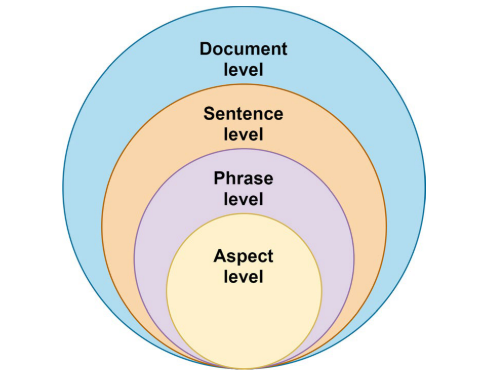
\includegraphics[scale=0.55]{images/dlengsteiner/sentimentanalasys_levels.png}
    \caption{Stufen der SA}
    \label{fig:sa-levels}
\end{figure}

Wie in Abbildung \ref{fig:sa-levels} gezeigt \cite[5734]{Wankhade2022sentiment}, wurde die Sentimentanalyse auf vier Stufen investigiert: Die \textbf{Dokument-Stufe}, die \textbf{Satz-Stufe}, die \textbf{Phrasen-Stufe} und die \textbf{Aspekt-Stufe}.

In \cite[21568]{amjad2023sentiment} werden nur drei Stufen genannt; Die Phrasen-Stufe wird nicht erwähnt. Ein möglicher Grund dafür wird später erläutert.

\paragraph{Dokument-Stufe:}

Hierbei wird dem gesamten Dokument eine Polarität vergeben \cite[5734]{Wankhade2022sentiment}\cite[21571]{amjad2023sentiment}. Das macht man, um eine Gesamtübersicht der Polarität eines Dokuments wie einer gesamten Review, einer Buchseite oder einem Kapitel zu bekommen. Es kann trotzdem sein, dass es Teile in dem Dokument gibt, welche negativ sind, es geht aber um die Gesamtheit des Dokuments. Diese Stufe der SA wird relativ selten verwendet.

Auf dieser Stufe lässt sich noch supervised Learning betreiben \cite[5734]{Wankhade2022sentiment}. Das liegt vermutlich daran, dass die Anzahl der Dokumente viel geringer ist als die Anzahl von zum Beispiel Sätzen, weswegen es relativ einfach und billig ist, Dokumente als Trainingsdaten manuell zu labeln.

\paragraph{Satz-Stufe:}

Mit dieser Stufe geht man spezifischer auf das Sentiment der Textdaten ein \cite[21572]{amjad2023sentiment}. Jeder Satz bekommt eine Polarität, wird also als positiv, neutral oder negativ eingestuft. Supervised Learning auf dieser Stufe ist weitaus aufwändiger \cite[5734]{Wankhade2022sentiment}. Die Polaritäten der Sätze können entweder zu einem Dokument aggregiert werden oder einzelnd betrachtet werden. Diese Stufe eignet sich somit besonders gut für Dokumente, welche mit verschiedensten Sentimenten assoziiert werden bzw. beinhalten.

Diese Stufe hat aber auch eine Schwäche \cite[5734-5735]{Wankhade2022sentiment}: Sowohl Sätze mit Abhängigkeiten von anderen Sätzen als auch mehrdeutige Aussagen sind schwer zuzuordnen, weswegen in solchen Fällen von der Satz-Stufe abgeraten wird. 

\paragraph{Phrasen-Stufe:}

Phrasen sind Wortgefüge, welche meistens kürzer als ein Satz sind und nicht als einer fungieren, wie in \cite[154]{Meibauer2003phrasen} mit Beispielen gezeigt wird.

Was die Satz-Stufe für die Dokument-Stufe ist, ist die Phrasen-Stufe für die Satz-Stufe \cite[5735]{Wankhade2022sentiment}: Die Satz-Stufe erlaubt es, mehrere Polaritäten in einem Dokument vorkommen zu lassen. Die Phrasen-Stufe wiederum erlaubt mehrere Polaritäten in einem Satz. Diese Stufe ist vor allem für Rezensionen, welche aus mehreren Zeilen bestehen, geeignet, wenn diese Zeilen nicht als ganze Sätze gelten.

\paragraph{Aspekt-Stufe:}

Diese Stufe ist die spezifischte Stufe \cite[21572]{amjad2023sentiment} und wird vor allem dann verwendet, wenn man ganz genau wissen möchte, was den Leuten gefallen hat und was nicht, zum Beispiel bei einem Produkt. Dazu kann man sich folgende ausgedachte Rezension als Beispiel ansehen:
\begin{quote}
    Ich mag das neue Feature XY der App, jedoch ist mir das neue Design zuwieder.
\end{quote}
Dieser Satz behandelt zwei Aspekte einer App: Das neue Feature XY sowie das Design. Die Polaritäten sind jedoch gegensätzlich. Mit der Satz-Stufe hätte man also Schwierigkeiten, diesen Satz einzuordnen.

Diese Stufe fokussiert sich nicht auf das Sentiment eines Satzes oder Absatzes, sondern auf \textbf{charakteristische Eigenschaften von Merkmalen}.

Der Grund, warum \cite{amjad2023sentiment} die Phrasen-Stufe ausgelassen hat, könnte also daran liegen, dass die Phrasen-Stufe als redundant gesehen wird. Im Grunde genommen tut sie nämlich fast genau dasselbe wie die Aspekt-Stufe, mit dem Unterschied, dass man sich noch auf das Sentiment und nicht auf Merkmale fokussiert.

\subsubsection{SA-Prozess}

Der generische Prozess für SA besteht aus fünf Schritten, wie in \ref{fig:sa-process} dargestellt \cite[21572]{amjad2023sentiment}. Es wird mit der Datensammlung begonnen. Dieser Schritt ist für dieses Projekt nicht allzu relevant. Danach beginnt das Pre-Processing. Hier werden die Daten für die weitere Verwendung aufbereitet. Danach ist die Feature-Extraction an der Reihe. In diesem Schritt sucht man sich die relevantesten Merkmale für den nächsten Schritt heraus. Dieser ist die Klassifizierung, in der die tatsächliche SA durchgeführt wird. Hier können unterschiedliche Herangehensweisen verwendet werden. Zu guter letzt gibt es die Performance-Evaluation, um bewerten zu können, wie effizient die Herangehensweise tatsächlich war.

\begin{figure}
    \centering
    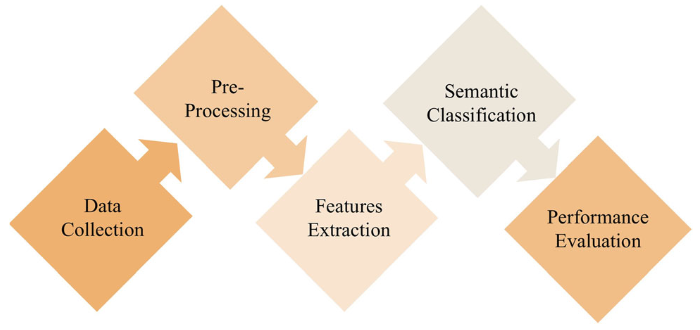
\includegraphics[scale=0.43]{images/dlengsteiner/sentimentanalasys_process.png}
    \caption{Schritte der SA}
    \label{fig:sa-process}
\end{figure}
